
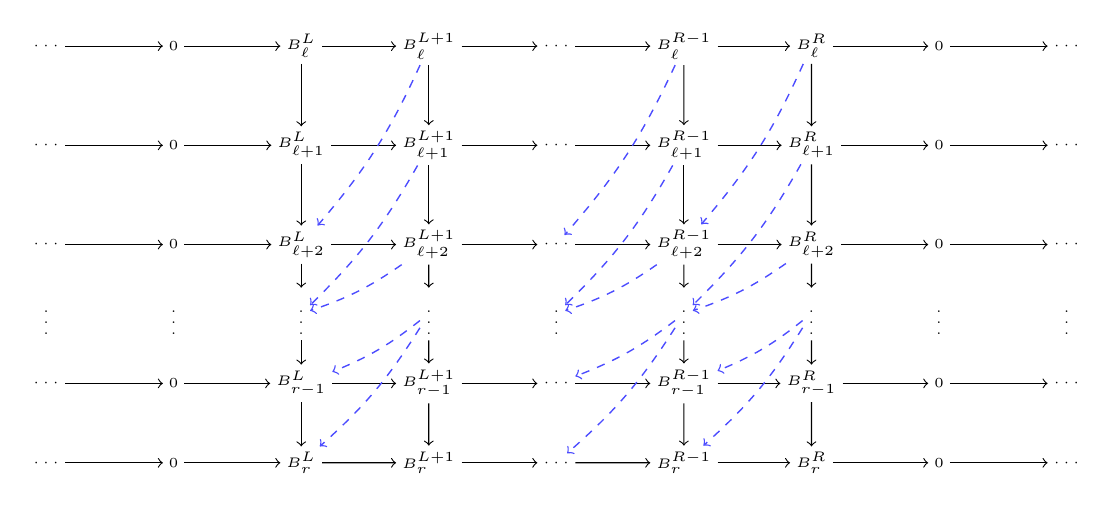
\begin{tikzpicture}[
  scale=0.9,
  every node/.style={
    inner sep=2pt,
    font=\tiny
  }
]
 
% Compact cochain complex style
\def\colspacing{1.8}
\def\rowspacing{1.4}
 
% ==========================================
% ROW 1: i = ℓ (top row)
% ==========================================
\node (A0_m1) at (-\colspacing, 0) {$\cdots$};
\node (A0_0) at (0, 0) {$0$};
\node (A0_1) at (\colspacing, 0) {$B_\ell^L$};
\node (A0_2) at (2*\colspacing, 0) {$B_\ell^{L+1}$};
\node (A0_3) at (3*\colspacing, 0) {$\cdots$};
\node (A0_4) at (4*\colspacing, 0) {$B_\ell^{R-1}$};
\node (A0_5) at (5*\colspacing, 0) {$B_\ell^R$};
\node (A0_6) at (6*\colspacing, 0) {$0$};
\node (A0_7) at (7*\colspacing, 0) {$\cdots$};
 
% ==========================================
% ROW 2: i = ℓ+1
% ==========================================
\node (A1_m1) at (-\colspacing, -\rowspacing) {$\cdots$};
\node (A1_0) at (0, -\rowspacing) {$0$};
\node (A1_1) at (\colspacing, -\rowspacing) {$B_{\ell+1}^L$};
\node (A1_2) at (2*\colspacing, -\rowspacing) {$B_{\ell+1}^{L+1}$};
\node (A1_3) at (3*\colspacing, -\rowspacing) {$\cdots$};
\node (A1_4) at (4*\colspacing, -\rowspacing) {$B_{\ell+1}^{R-1}$};
\node (A1_5) at (5*\colspacing, -\rowspacing) {$B_{\ell+1}^R$};
\node (A1_6) at (6*\colspacing, -\rowspacing) {$0$};
\node (A1_7) at (7*\colspacing, -\rowspacing) {$\cdots$};
 
% ==========================================
% ROW 3: i = ℓ+2
% ==========================================
\node (A2_m1) at (-\colspacing, -2*\rowspacing) {$\cdots$};
\node (A2_0) at (0, -2*\rowspacing) {$0$};
\node (A2_1) at (\colspacing, -2*\rowspacing) {$B_{\ell+2}^L$};
\node (A2_2) at (2*\colspacing, -2*\rowspacing) {$B_{\ell+2}^{L+1}$};
\node (A2_3) at (3*\colspacing, -2*\rowspacing) {$\cdots$};
\node (A2_4) at (4*\colspacing, -2*\rowspacing) {$B_{\ell+2}^{R-1}$};
\node (A2_5) at (5*\colspacing, -2*\rowspacing) {$B_{\ell+2}^R$};
\node (A2_6) at (6*\colspacing, -2*\rowspacing) {$0$};
\node (A2_7) at (7*\colspacing, -2*\rowspacing) {$\cdots$};
 
% ==========================================
% VERTICAL ELLIPSIS ROW (rows ℓ+3 through r-2)
% ==========================================
\node (vdots_m1) at (-\colspacing, -2.7*\rowspacing) {$\vdots$};
\node (vdots_0) at (0, -2.7*\rowspacing) {$\vdots$};
\node (vdots_1) at (\colspacing, -2.7*\rowspacing) {$\vdots$};
\node (vdots_2) at (2*\colspacing, -2.7*\rowspacing) {$\vdots$};
\node (vdots_3) at (3*\colspacing, -2.7*\rowspacing) {$\vdots$};
\node (vdots_4) at (4*\colspacing, -2.7*\rowspacing) {$\vdots$};
\node (vdots_5) at (5*\colspacing, -2.7*\rowspacing) {$\vdots$};
\node (vdots_6) at (6*\colspacing, -2.7*\rowspacing) {$\vdots$};
\node (vdots_7) at (7*\colspacing, -2.7*\rowspacing) {$\vdots$};
 
% ==========================================
% ROW r-1
% ==========================================
\node (A3_m1) at (-\colspacing, -3.4*\rowspacing) {$\cdots$};
\node (A3_0) at (0, -3.4*\rowspacing) {$0$};
\node (A3_1) at (\colspacing, -3.4*\rowspacing) {$B_{r-1}^L$};
\node (A3_2) at (2*\colspacing, -3.4*\rowspacing) {$B_{r-1}^{L+1}$};
\node (A3_3) at (3*\colspacing, -3.4*\rowspacing) {$\cdots$};
\node (A3_4) at (4*\colspacing, -3.4*\rowspacing) {$B_{r-1}^{R-1}$};
\node (A3_5) at (5*\colspacing, -3.4*\rowspacing) {$B_{r-1}^R$};
\node (A3_6) at (6*\colspacing, -3.4*\rowspacing) {$0$};
\node (A3_7) at (7*\colspacing, -3.4*\rowspacing) {$\cdots$};
 
% ==========================================
% ROW r (bottom row)
% ==========================================
\node (A4_m1) at (-\colspacing, -4.2*\rowspacing) {$\cdots$};
\node (A4_0) at (0, -4.2*\rowspacing) {$0$};
\node (A4_1) at (\colspacing, -4.2*\rowspacing) {$B_r^L$};
\node (A4_2) at (2*\colspacing, -4.2*\rowspacing) {$B_r^{L+1}$};
\node (A4_3) at (3*\colspacing, -4.2*\rowspacing) {$\cdots$};
\node (A4_4) at (4*\colspacing, -4.2*\rowspacing) {$B_r^{R-1}$};
\node (A4_5) at (5*\colspacing, -4.2*\rowspacing) {$B_r^R$};
\node (A4_6) at (6*\colspacing, -4.2*\rowspacing) {$0$};
\node (A4_7) at (7*\colspacing, -4.2*\rowspacing) {$\cdots$};
 
% ==========================================
% HORIZONTAL MAPS (along rows) - compact arrows
% ==========================================
 
% Row ℓ
\draw[->] (A0_m1) -- (A0_0);
\draw[->] (A0_0) -- (A0_1);
\draw[->] (A0_1) -- (A0_2);
\draw[->] (A0_2) -- (A0_3);
\draw[->] (A0_3) -- (A0_4);
\draw[->] (A0_4) -- (A0_5);
\draw[->] (A0_5) -- (A0_6);
\draw[->] (A0_6) -- (A0_7);
 
% Row ℓ+1
\draw[->] (A1_m1) -- (A1_0);
\draw[->] (A1_0) -- (A1_1);
\draw[->] (A1_1) -- (A1_2);
\draw[->] (A1_2) -- (A1_3);
\draw[->] (A1_3) -- (A1_4);
\draw[->] (A1_4) -- (A1_5);
\draw[->] (A1_5) -- (A1_6);
\draw[->] (A1_6) -- (A1_7);
 
% Row ℓ+2
\draw[->] (A2_m1) -- (A2_0);
\draw[->] (A2_0) -- (A2_1);
\draw[->] (A2_1) -- (A2_2);
\draw[->] (A2_2) -- (A2_3);
\draw[->] (A2_3) -- (A2_4);
\draw[->] (A2_4) -- (A2_5);
\draw[->] (A2_5) -- (A2_6);
\draw[->] (A2_6) -- (A2_7);
 
% Row r-1
\draw[->] (A3_m1) -- (A3_0);
\draw[->] (A3_0) -- (A3_1);
\draw[->] (A3_1) -- (A3_2);
\draw[->] (A3_2) -- (A3_3);
\draw[->] (A3_3) -- (A3_4);
\draw[->] (A3_4) -- (A3_5);
\draw[->] (A3_5) -- (A3_6);
\draw[->] (A3_6) -- (A3_7);
 
% Row r
\draw[->] (A4_m1) -- (A4_0);
\draw[->] (A4_0) -- (A4_1);
\draw[->] (A4_1) -- (A4_2);
\draw[->] (A4_2) -- (A4_3);
\draw[->] (A4_3) -- (A4_4);
\draw[->] (A4_4) -- (A4_5);
\draw[->] (A4_5) -- (A4_6);
\draw[->] (A4_6) -- (A4_7);
 
% ==========================================
% VERTICAL MAPS (along columns)
% ==========================================
 
% Column L (leftmost)
\draw[->] (A0_1) -- (A1_1);
\draw[->] (A1_1) -- (A2_1);
\draw[->] (A2_1) -- (vdots_1);
\draw[->] (vdots_1) -- (A3_1);
\draw[->] (A3_1) -- (A4_1);
 
% Column L+1
\draw[->] (A0_2) -- (A1_2);
\draw[->] (A1_2) -- (A2_2);
\draw[->] (A2_2) -- (vdots_2);
\draw[->] (vdots_2) -- (A3_2);
\draw[->] (A3_2) -- (A4_2);
 
% Column R-1
\draw[->] (A0_4) -- (A1_4);
\draw[->] (A1_4) -- (A2_4);
\draw[->] (A2_4) -- (vdots_4);
\draw[->] (vdots_4) -- (A3_4);
\draw[->] (A3_4) -- (A4_4);
 
% Column R
\draw[->] (A0_5) -- (A1_5);
\draw[->] (A1_5) -- (A2_5);
\draw[->] (A2_5) -- (vdots_5);
\draw[->] (vdots_5) -- (A3_5);
\draw[->] (A3_5) -- (A4_5);
 
% ==========================================
% DIAGONAL MAPS: B_i^j → B_{i+2}^{j-1}
% From all columns L+1, L+2, ..., R
% Rows ℓ and ℓ+1 map to row ℓ+2
% Row ℓ+2 maps to ellipsis row
% Ellipsis row maps to rows r-1 and r
% ==========================================
 
% From row ℓ:
% A0_2 (L+1) -> A2_1 (L)
\draw[
  ->,
  dashed,
  line width=0.5pt,
  color=blue!70
] (A0_2) to[bend left=8] (A2_1);
 
% A0_4 (R-1) -> A2_3 (R-2, the ellipsis)
\draw[
  ->,
  dashed,
  line width=0.5pt,
  color=blue!70
] (A0_4) to[bend left=8] (A2_3);
 
% A0_5 (R) -> A2_4 (R-1)
\draw[
  ->,
  dashed,
  line width=0.5pt,
  color=blue!70
] (A0_5) to[bend left=8] (A2_4);
 
% From row ℓ+1:
% A1_2 (L+1) -> vdots_1 (L) in ellipsis row
\draw[
  ->,
  dashed,
  line width=0.5pt,
  color=blue!70
] (A1_2) to[bend left=8] (vdots_1);
 
% A1_4 (R-1) -> vdots_3 (R-2)
\draw[
  ->,
  dashed,
  line width=0.5pt,
  color=blue!70
] (A1_4) to[bend left=8] (vdots_3);
 
% A1_5 (R) -> vdots_4 (R-1)
\draw[
  ->,
  dashed,
  line width=0.5pt,
  color=blue!70
] (A1_5) to[bend left=8] (vdots_4);
 
% From row ℓ+2:
% A2_2 (L+1) -> vdots_1 (L) in ellipsis row
\draw[
  ->,
  dashed,
  line width=0.5pt,
  color=blue!70
] (A2_2) to[bend left=8] (vdots_1);
 
% A2_4 (R-1) -> vdots_3 (R-2) in ellipsis row
\draw[
  ->,
  dashed,
  line width=0.5pt,
  color=blue!70
] (A2_4) to[bend left=8] (vdots_3);
 
% A2_5 (R) -> vdots_4 (R-1) in ellipsis row
\draw[
  ->,
  dashed,
  line width=0.5pt,
  color=blue!70
] (A2_5) to[bend left=8] (vdots_4);
 
% From ellipsis row to row r-1:
% vdots_2 (L+1) -> A3_1 (L)
\draw[
  ->,
  dashed,
  line width=0.5pt,
  color=blue!70
] (vdots_2) to[bend left=8] (A3_1);
 
% vdots_4 (R-1) -> A3_3 (R-2, the ellipsis)
\draw[
  ->,
  dashed,
  line width=0.5pt,
  color=blue!70
] (vdots_4) to[bend left=8] (A3_3);
 
% vdots_5 (R) -> A3_4 (R-1)
\draw[
  ->,
  dashed,
  line width=0.5pt,
  color=blue!70
] (vdots_5) to[bend left=8] (A3_4);
 
% From ellipsis row to row r:
% vdots_2 (L+1) -> A4_1 (L)
\draw[
  ->,
  dashed,
  line width=0.5pt,
  color=blue!70
] (vdots_2) to[bend left=8] (A4_1);
 
% vdots_4 (R-1) -> A4_3 (R-2, the ellipsis)
\draw[
  ->,
  dashed,
  line width=0.5pt,
  color=blue!70
] (vdots_4) to[bend left=8] (A4_3);
 
% vdots_5 (R) -> A4_4 (R-1)
\draw[
  ->,
  dashed,
  line width=0.5pt,
  color=blue!70
] (vdots_5) to[bend left=8] (A4_4);
 
\end{tikzpicture}